\chapter{感知机数学模型}
\label{chap:math_perceptron}

\section{感知机}

弄清感知机(Perceptron)是学好支持向量机和神经网络的基础。可以把感知机看成n维实例空间的决策超平面:W*X=0.这个超平面将空间中的点分为正负两类。如果给定的数据集线性可分,则可以将每个样例准确地分为两类,称为分类超平面。而其中(w1,w2,...,wn)为这个超平面的法向量,w0称为截距。

\begin{figure}[!htb]
\centering
\begin{tikzpicture}[node distance=1cm]
%定义流程图具体形状
\node[perceptron](circle){$\Sigma$};
%连接具体形状
\node[left of=circle,xshift=-2cm,yshift=1cm,draw=none,fill=none](x1){x1};
\node[left of=circle,xshift=-2cm, draw=none,fill=none](x2){x2};
\node[left of=circle,xshift=-2cm,yshift=-1cm, draw=none,fill=none](x3){x3};
\node[right of=circle,xshift=2cm,draw=none,fill=none](output){output};
\draw [arrow](x1) -- (circle);
\draw [arrow](x2) -- (circle);
\draw [arrow](x3) -- (circle);
\draw [arrow](circle)--(output);
\end{tikzpicture}
\caption{感知机模型}
\label{fig:part2_math_perceptron_module}
\end{figure}


\begin{equation}
f(x) = 
\begin{cases}
1 & \text{如果 $W\cdot X+b > 0$}\\
0 & \text{其它}
\end{cases}
\label{part2_math_perceptron_formula}
\end{equation}

\ \\ \noindent
\eqnref{part2_math_perceptron_formula},w和b为感知机参数,w为权值(weight),b为偏置(bias)。

\ \\ \noindent
使用\emph{感知机}可解决线性可分问题,对于XOR问题就无法解决,如\figref{fig:part2_perceptron_logical}说明了这个原因。
其中,输入$X$为: $(0,0),(0,1),(1,0),(1,1)$,期望获得正确输出。

\begin{figure}[!htb]
\centerline{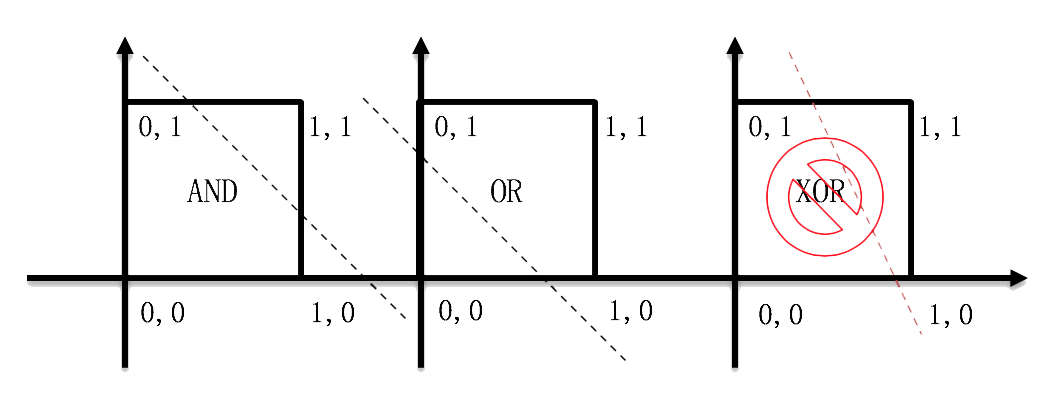
\includegraphics[width=.4\figwidth]{images/logical.png}}
\label{fig:part2_perceptron_logical}
\caption{感知机解决逻辑问题}
\end{figure}

\ \\
异或的问题暂且不用例会,感知机在线性可分问题上还是绰绰有余的!



\section{SVM支持向量机}


\section{卷积神经网络}




